% Title: glps_renderer figure
% Creator: GL2PS 1.3.8, (C) 1999-2012 C. Geuzaine
% For: Octave
% CreationDate: Fri Oct 21 17:46:43 2016
\setlength{\unitlength}{1pt}
\begin{picture}(0,0)
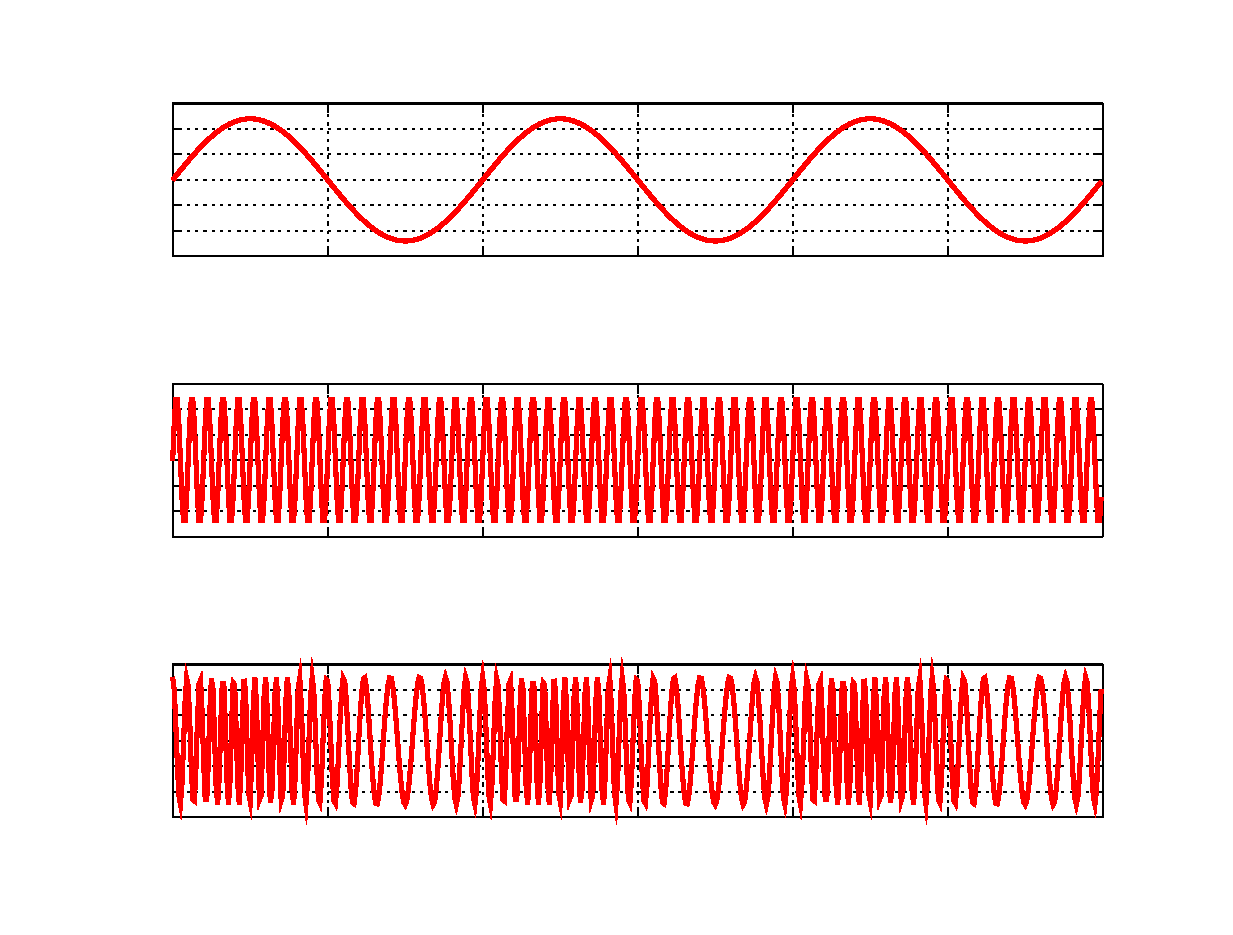
\includegraphics{fm-inc}
\end{picture}%
\begin{picture}(576,433)(0,0)
\fontsize{10}{0}
\selectfont\put(74.88,312.778){\makebox(0,0)[t]{\textcolor[rgb]{0,0,0}{{0}}}}
\fontsize{10}{0}
\selectfont\put(149.28,312.778){\makebox(0,0)[t]{\textcolor[rgb]{0,0,0}{{0.01}}}}
\fontsize{10}{0}
\selectfont\put(223.68,312.778){\makebox(0,0)[t]{\textcolor[rgb]{0,0,0}{{0.02}}}}
\fontsize{10}{0}
\selectfont\put(298.08,312.778){\makebox(0,0)[t]{\textcolor[rgb]{0,0,0}{{0.03}}}}
\fontsize{10}{0}
\selectfont\put(372.48,312.778){\makebox(0,0)[t]{\textcolor[rgb]{0,0,0}{{0.04}}}}
\fontsize{10}{0}
\selectfont\put(446.88,312.778){\makebox(0,0)[t]{\textcolor[rgb]{0,0,0}{{0.05}}}}
\fontsize{10}{0}
\selectfont\put(521.28,312.778){\makebox(0,0)[t]{\textcolor[rgb]{0,0,0}{{0.06}}}}
\fontsize{10}{0}
\selectfont\put(69.8755,317.799){\makebox(0,0)[r]{\textcolor[rgb]{0,0,0}{{-15}}}}
\fontsize{10}{0}
\selectfont\put(69.8755,330.02){\makebox(0,0)[r]{\textcolor[rgb]{0,0,0}{{-10}}}}
\fontsize{10}{0}
\selectfont\put(69.8755,342.24){\makebox(0,0)[r]{\textcolor[rgb]{0,0,0}{{-5}}}}
\fontsize{10}{0}
\selectfont\put(69.8755,354.46){\makebox(0,0)[r]{\textcolor[rgb]{0,0,0}{{0}}}}
\fontsize{10}{0}
\selectfont\put(69.8755,366.68){\makebox(0,0)[r]{\textcolor[rgb]{0,0,0}{{5}}}}
\fontsize{10}{0}
\selectfont\put(69.8755,378.9){\makebox(0,0)[r]{\textcolor[rgb]{0,0,0}{{10}}}}
\fontsize{10}{0}
\selectfont\put(69.8755,391.12){\makebox(0,0)[r]{\textcolor[rgb]{0,0,0}{{15}}}}
\fontsize{10}{0}
\selectfont\put(298.08,301.778){\makebox(0,0)[t]{\textcolor[rgb]{0,0,0}{{\frac{t}{s}}}}}
\fontsize{10}{0}
\selectfont\put(74.88,178.138){\makebox(0,0)[t]{\textcolor[rgb]{0,0,0}{{0}}}}
\fontsize{10}{0}
\selectfont\put(149.28,178.138){\makebox(0,0)[t]{\textcolor[rgb]{0,0,0}{{0.01}}}}
\fontsize{10}{0}
\selectfont\put(223.68,178.138){\makebox(0,0)[t]{\textcolor[rgb]{0,0,0}{{0.02}}}}
\fontsize{10}{0}
\selectfont\put(298.08,178.138){\makebox(0,0)[t]{\textcolor[rgb]{0,0,0}{{0.03}}}}
\fontsize{10}{0}
\selectfont\put(372.48,178.138){\makebox(0,0)[t]{\textcolor[rgb]{0,0,0}{{0.04}}}}
\fontsize{10}{0}
\selectfont\put(446.88,178.138){\makebox(0,0)[t]{\textcolor[rgb]{0,0,0}{{0.05}}}}
\fontsize{10}{0}
\selectfont\put(521.28,178.138){\makebox(0,0)[t]{\textcolor[rgb]{0,0,0}{{0.06}}}}
\fontsize{10}{0}
\selectfont\put(69.8755,183.16){\makebox(0,0)[r]{\textcolor[rgb]{0,0,0}{{-6}}}}
\fontsize{10}{0}
\selectfont\put(69.8755,195.38){\makebox(0,0)[r]{\textcolor[rgb]{0,0,0}{{-4}}}}
\fontsize{10}{0}
\selectfont\put(69.8755,207.6){\makebox(0,0)[r]{\textcolor[rgb]{0,0,0}{{-2}}}}
\fontsize{10}{0}
\selectfont\put(69.8755,219.82){\makebox(0,0)[r]{\textcolor[rgb]{0,0,0}{{0}}}}
\fontsize{10}{0}
\selectfont\put(69.8755,232.04){\makebox(0,0)[r]{\textcolor[rgb]{0,0,0}{{2}}}}
\fontsize{10}{0}
\selectfont\put(69.8755,244.26){\makebox(0,0)[r]{\textcolor[rgb]{0,0,0}{{4}}}}
\fontsize{10}{0}
\selectfont\put(69.8755,256.48){\makebox(0,0)[r]{\textcolor[rgb]{0,0,0}{{6}}}}
\fontsize{10}{0}
\selectfont\put(298.08,167.138){\makebox(0,0)[t]{\textcolor[rgb]{0,0,0}{{\frac{t}{s}}}}}
\fontsize{10}{0}
\selectfont\put(74.88,43.498){\makebox(0,0)[t]{\textcolor[rgb]{0,0,0}{{0}}}}
\fontsize{10}{0}
\selectfont\put(149.28,43.498){\makebox(0,0)[t]{\textcolor[rgb]{0,0,0}{{0.01}}}}
\fontsize{10}{0}
\selectfont\put(223.68,43.498){\makebox(0,0)[t]{\textcolor[rgb]{0,0,0}{{0.02}}}}
\fontsize{10}{0}
\selectfont\put(298.08,43.498){\makebox(0,0)[t]{\textcolor[rgb]{0,0,0}{{0.03}}}}
\fontsize{10}{0}
\selectfont\put(372.48,43.498){\makebox(0,0)[t]{\textcolor[rgb]{0,0,0}{{0.04}}}}
\fontsize{10}{0}
\selectfont\put(446.88,43.498){\makebox(0,0)[t]{\textcolor[rgb]{0,0,0}{{0.05}}}}
\fontsize{10}{0}
\selectfont\put(521.28,43.498){\makebox(0,0)[t]{\textcolor[rgb]{0,0,0}{{0.06}}}}
\fontsize{10}{0}
\selectfont\put(69.8755,48.52){\makebox(0,0)[r]{\textcolor[rgb]{0,0,0}{{-6}}}}
\fontsize{10}{0}
\selectfont\put(69.8755,60.74){\makebox(0,0)[r]{\textcolor[rgb]{0,0,0}{{-4}}}}
\fontsize{10}{0}
\selectfont\put(69.8755,72.96){\makebox(0,0)[r]{\textcolor[rgb]{0,0,0}{{-2}}}}
\fontsize{10}{0}
\selectfont\put(69.8755,85.18){\makebox(0,0)[r]{\textcolor[rgb]{0,0,0}{{0}}}}
\fontsize{10}{0}
\selectfont\put(69.8755,97.4001){\makebox(0,0)[r]{\textcolor[rgb]{0,0,0}{{2}}}}
\fontsize{10}{0}
\selectfont\put(69.8755,109.62){\makebox(0,0)[r]{\textcolor[rgb]{0,0,0}{{4}}}}
\fontsize{10}{0}
\selectfont\put(69.8755,121.84){\makebox(0,0)[r]{\textcolor[rgb]{0,0,0}{{6}}}}
\fontsize{10}{0}
\selectfont\put(298.08,32.4981){\makebox(0,0)[t]{\textcolor[rgb]{0,0,0}{{\frac{t}{s}}}}}
\fontsize{10}{0}
\selectfont\put(298.08,401.12){\makebox(0,0)[b]{\textcolor[rgb]{0,0,0}{{Nachrichtensignal}}}}
\fontsize{10}{0}
\selectfont\put(298.08,266.48){\makebox(0,0)[b]{\textcolor[rgb]{0,0,0}{{Trägersignal}}}}
\fontsize{10}{0}
\selectfont\put(298.08,131.84){\makebox(0,0)[b]{\textcolor[rgb]{0,0,0}{{Frequenzmodulieres Signal}}}}
\end{picture}
